
% asset_id: FAS1VectorsTikZ-003
% asset_type: tikz
% topic_id: FAS1Vectors
% unit_code: FAS1
% topic_code: FAS1-VEC
% related_lesson_file: FAS1_vectors_lesson.md
% related_lesson_section: # 9. Visual Asset Integration
% source: FP1-Chp1-Vectors.pdf + transcripts.md where relevant
\documentclass[tikz,border=8pt]{standalone}
\usepackage{amsmath}
\usepackage{xcolor}
\usetikzlibrary{arrows.meta,calc,positioning}
\definecolor{Canvas}{HTML}{FAF9F6}
\definecolor{Ivory}{HTML}{FFFFF0}
\definecolor{LineGrey}{HTML}{E5E5EA}
\definecolor{Gold}{HTML}{C5A059}
\definecolor{TextInk}{HTML}{2C2C2E}
\definecolor{SoftPink}{HTML}{FBEFEF}
\begin{document}
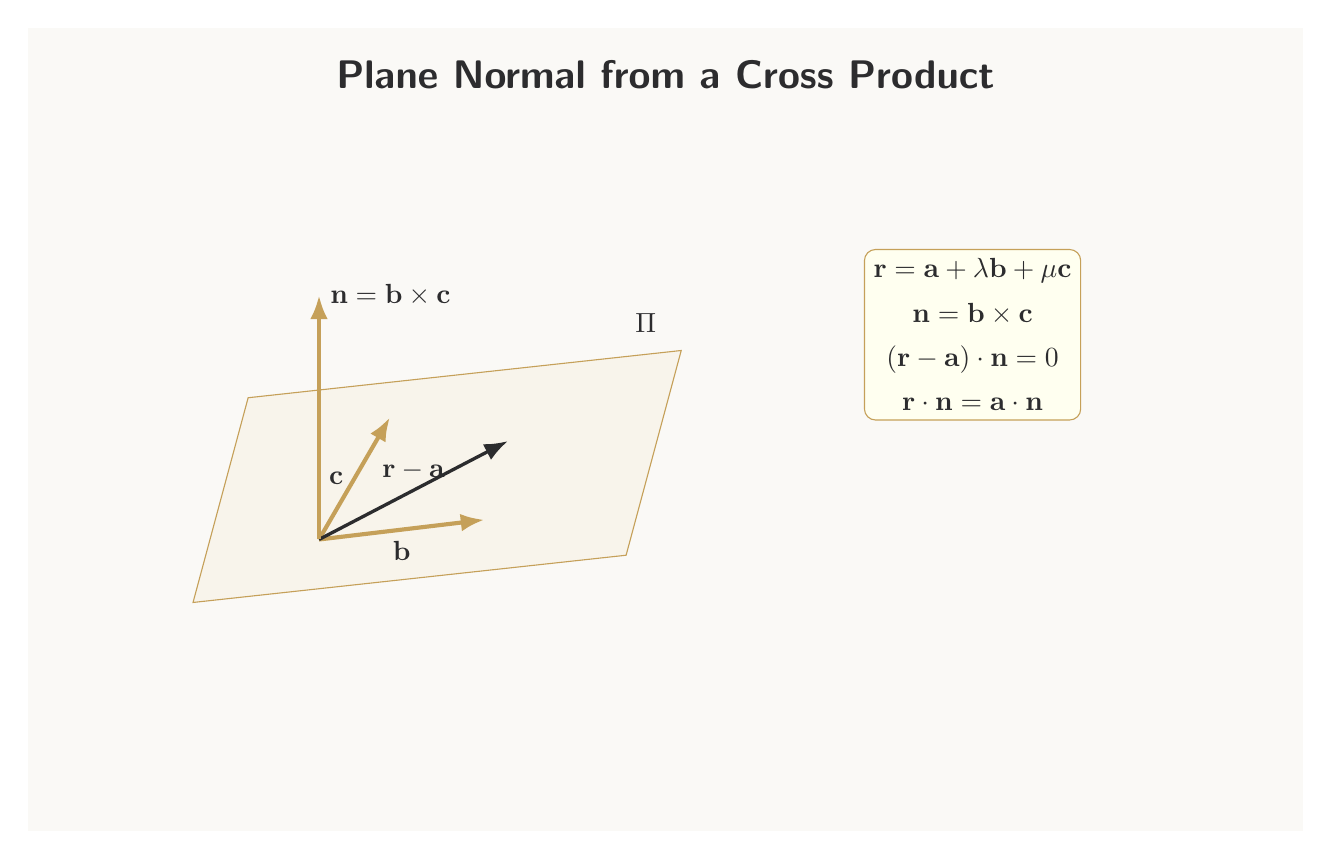
\begin{tikzpicture}[every node/.style={font=\sffamily,text=TextInk},arrow/.style={-{Latex[length=3mm]},line width=1.2pt,draw=TextInk},goldarrow/.style={-{Latex[length=3mm]},line width=1.5pt,draw=Gold}]
\fill[Canvas] (-0.6,-0.6) rectangle (15.6,9.6);

\node[font=\sffamily\bfseries\Large] at (7.5,9) {Plane Normal from a Cross Product};
\coordinate (P0) at (1.5,2.3); \coordinate (P1) at (7,2.9); \coordinate (P2) at (7.7,5.5); \coordinate (P3) at (2.2,4.9);
\filldraw[fill=Gold!12,draw=Gold] (P0)--(P1)--(P2)--(P3)--cycle; \node at (7.25,5.85) {$\Pi$};
\coordinate (A) at (3.1,3.1); \coordinate (Bv) at (5.2,3.35); \coordinate (Cv) at (4.0,4.65); \coordinate (R) at (5.5,4.35);
\draw[goldarrow] (A)--(Bv) node[midway,below] {$\mathbf b$}; \draw[goldarrow] (A)--(Cv) node[midway,left] {$\mathbf c$}; \draw[arrow] (A)--(R) node[midway,above] {$\mathbf r-\mathbf a$}; \draw[goldarrow] (A)--++(0,3.1) node[right] {$\mathbf n=\mathbf b\times\mathbf c$};
\node[draw=Gold,fill=Ivory,rounded corners,align=center] at (11.4,5.7) {$\mathbf r=\mathbf a+\lambda\mathbf b+\mu\mathbf c$\\[4pt]$\mathbf n=\mathbf b\times\mathbf c$\\[4pt]$(\mathbf r-\mathbf a)\cdot\mathbf n=0$\\[4pt]$\mathbf r\cdot\mathbf n=\mathbf a\cdot\mathbf n$};

\end{tikzpicture}
\end{document}
